%%%%%%%%%%%%%%%%%%%%%%%%%%%%%%%%%%%%%%%%%%%%%%%%%%%%
% This will help you in writing your homebook
% Remember that the character % is a comment in latex
%
% chapter 1

\chapter{Reference model development}
\label{chap1}
\graphicspath{ {./chapters/chap1images/} }
%%%%%%%%%%%%%%%%%%%%%%%%%%%%%%%%%%%%%%%%%%%%%%%%%%%%%%%%%%%
% you can organize a chapter using sections -> \section{Simulating an inverter}
% or subsections -> \subsection{simulating a particular type of inverter}
%%%%%%   First section
\section{Introduction}

The goal of this laboratory is to design a Finite Impulse Filter filter (FIR) with a cut frequency of 2 kHz, and then applying some optimization 
techniques such as unfolding and pipelining to the basic structure.
Filter was designed according two parameter: order and number of bits. The order employed for the following filter
is 10 and the number of bits is 9.
A prototype version of the filter has been developed in C language and Matlab in order to be able to compare their results with the
ones coming from the simulation of the HDL design.
%\paragraph{}
In the following table the main filter specifications are summarized:
%\paragraph{}

%\centerline{
%\begin{tabular}{ |p{3cm}||p{3cm}|p{3cm}|p{3cm}|  }
%	\hline
%	Filter Specification&Value \\
%	\hline
%	Filter Type   & FIR filter\\
%	Cut-off frequency&   2kHz\\
%	Sampling frequency &10kHz\\
%	Filter order    &10\\
%	Number of bits&   9\\
%	\hline
%   \end{tabular}}
%
%\section{Design the filter with Matlab}

\paragraph{}
\centerline{
	\begin{tabularx}{0.8\textwidth} { 
	| >{\centering\arraybackslash}X  
	| >{\centering\arraybackslash}X | }
	\hline
	\textbf{Filter Specification} & \textbf{Value} \\
	\hline
	Filter Type & FIR filter\\
	\hline
	Cut-off frequency & 2kHz\\
	\hline
	Sampling frequency & 10kHz\\
	\hline
	Filter order & 10\\
	\hline
	Number of bits & 9\\
	\hline
	\end{tabularx}
}

\paragraph{}

First step is the generation of coefficients. To do this Matlab function fir1 has been used.
The coefficients are shown in the following table: %\ref{tab:1}. % here is the reference to the table below
\paragraph{}
\centerline{
	\begin{tabularx}{0.8\textwidth} { 
	| >{\centering\arraybackslash}X 
	| >{\centering\arraybackslash}X 
	| >{\centering\arraybackslash}X | }
	\hline
	\textbf{Number} & \textbf{Integers} & \textbf{Normalized} \\
	\hline
	0 & -1 & -0.0078125 \\
	\hline
	1 & -2 & -0.015625 \\
	\hline
	2 & -4 & -0.03125 \\
	\hline
	3 & 8 & 0.0625 \\
	\hline
	4 & 35 & 0.2734375 \\
	\hline
	5 & 50 & 0.390625 \\
	\hline
	6 & 35 & 0.2734375 \\
	\hline
	7 & 8 & 0.0625 \\
	\hline
	8 & -4 & -0.03125 \\
	\hline
	9 & -2 & -0.015625 \\
	\hline
	10 & -1 & -0.0078125 \\
	\hline
	\end{tabularx}
}

%\begin{table}%[ht]
%\centering
%\begin{tabular}{c|c|c}
%\toprule
%Number & Integers & Normalized \\
%\midrule
%0 & -1 & -0.0078125 \\
%1 & -2 & -0.015625 \\
%2 & -4 & -0.03125 \\
%3 & 8 & 0.0625 \\
%4 & 35 & 0.2734375 \\
%5 & 50 & 0.390625 \\
%6 & 35 & 0.2734375 \\
%7 & 8 & 0.0625 \\
%8 & -4 & -0.03125 \\
%9 & -2 & -0.015625 \\
%10 & -1 & -0.0078125 \\
%\bottomrule
%\end{tabular}
%\caption{All coefficients.}
%\label{tab:1}
%\end{table}
\paragraph{}
Those coefficients are subjected to a quantization operation over Nb bits and expressed both in integer and real form.
It is possible to esimate the effect of this quantization by comparing the designed transfer function to the quantized one, as shown in the following figure: %\ref{fig:1}.
\begin{figure}[!ht]
	%\caption{Designed Transfer Function vs Quantized Transfer Function}
	%\label{fig:1}
	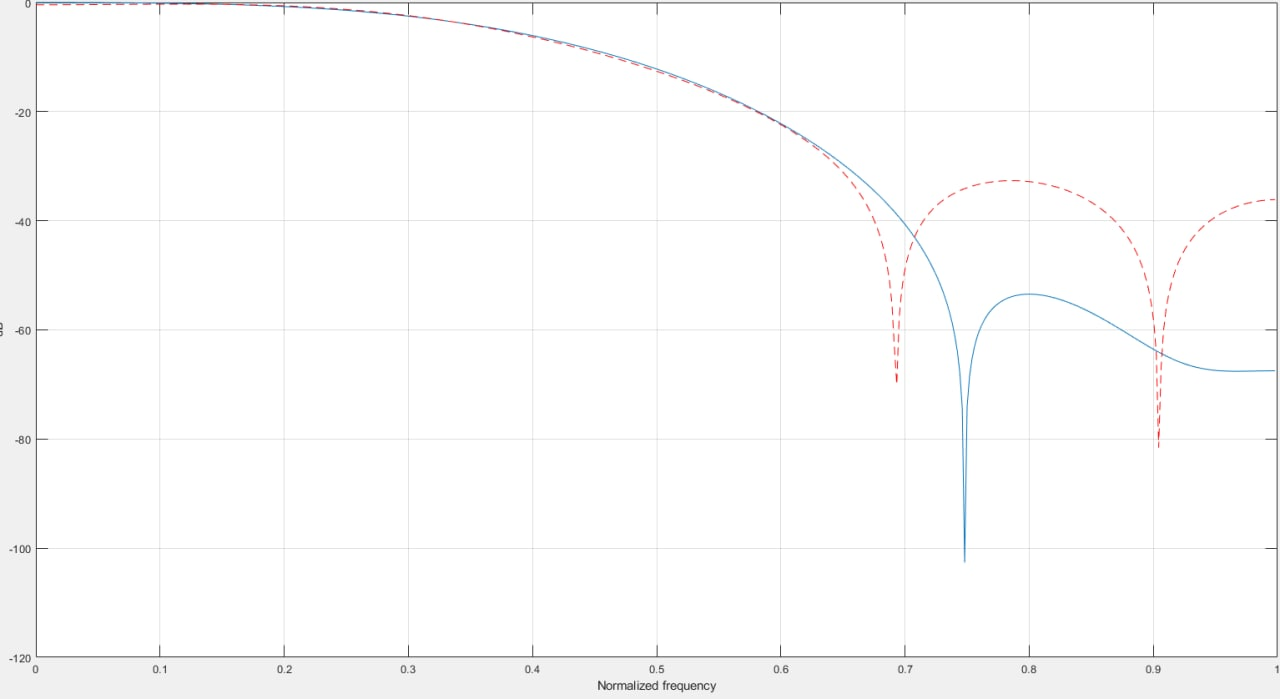
\includegraphics[width=15.5cm]{IMG1.jpg}
	\centering
\end{figure}

\paragraph{}
At this point, another Matlab script is executed in order to perform
different simulatios with prototype filter with a cut-off frequency of 2 kHz and a sampling frequency of 10 kHz, taking as 
input signal the average value between two sinusoidal waves of frequency of 500 HZ and 4.5 kHz respectively.
After this execution two files have been generated:

\begin{enumerate}
	\item \emph{sample.txt}, which contains the sample values that have fed the input of the FIR;
	\item \emph{result.txt}, which contains the output values that has been elaborated from the FIR.
\end{enumerate}

The following figure shows the two sinusoidal waveforms and the effective filter's input:
\begin{figure}[!ht]
	%\caption{FIR Input and Output overt time}
	%\label{fig:2}
	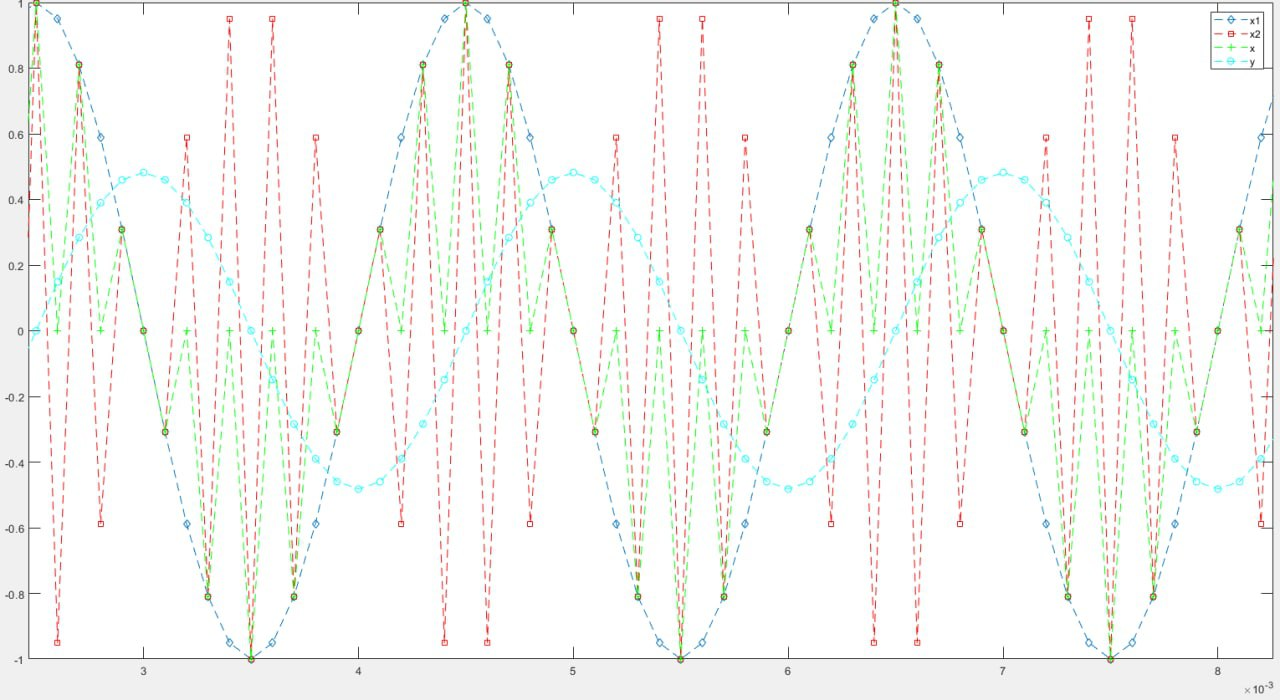
\includegraphics[scale=0.35]{IMG2.jpg}
	\centering
\end{figure}


\section{C prototype}

The C-language script simualtes a FIR filter implementing the following  relation:

\begin{displaymath}[!h]
y_i = \sum_{n=0}^{10}{x_{i-n} \cdot b_n}
\end{displaymath}
\paragraph{}
Inside the script, a function is defined in order to evaluate the output y[n] at a specific time instant, knowing the input sample x[n].
\paragraph{}
FIR constants are hardcoded inside the script, declared as a constant array of integers, while an internal buffer is needed to store the previous input values and shift them for each function call, and the output is obtained by summing coefficient-input products in a loop.
\paragraph{}
In order to emulate the finite internal parallelism of the hardware architecture, a shift operation is performed on the result before storing it into the accumulator.
Of course, this truncation operation introduces an error in the evaluation of the output samples.
The maximum accurancy would be obtained with a parallelism that is equale to the double of the bits number used for the architecture.

\paragraph{}
Thanks to this script is possible to compare the performance of the fixed-point version with respect to 
the Matlab computation results.

\subsection{Evaluate the THD}

The purpose of this step is to evaluate the Total Harmonic Distortion (THD), trying to obtain a maximum 
value of -30dB. 
\paragraph{}
If THD exceeds the maximum tolerated value, it is necessary to increase 
the bit numbers in order to reduce its amount, while if there is a gap between the maximum tolerated value 
and the obtained one, it is possible to reduce bit numbers and thus the complexity of the FIR implementation.
%% add value of THD caculated each time
\paragraph{}
With 9 bits used for data, obtained THD is -39.07 dB. 
Reducing the number of bits to 8 the obtained value of THD  
is -33.65 dB, thus still acceptable. 
Applying a further bit-number reduction, thus with a 7-bit parallelism, the value of THD exceeds the maximum allowed
amount, reaching the value of -27.01 dB.
\paragraph{}
At the end of this analysis, it has been decided to use 8 bits for the final implementation of the  FIR, 
in order to reduce the area while still accomplish the requested THD amount, shown in the following figure: %\ref{fig:3}.
\begin{figure}[!h]
	%\caption{Final THD for FIR filter implementation}
	%\label{fig:3}
	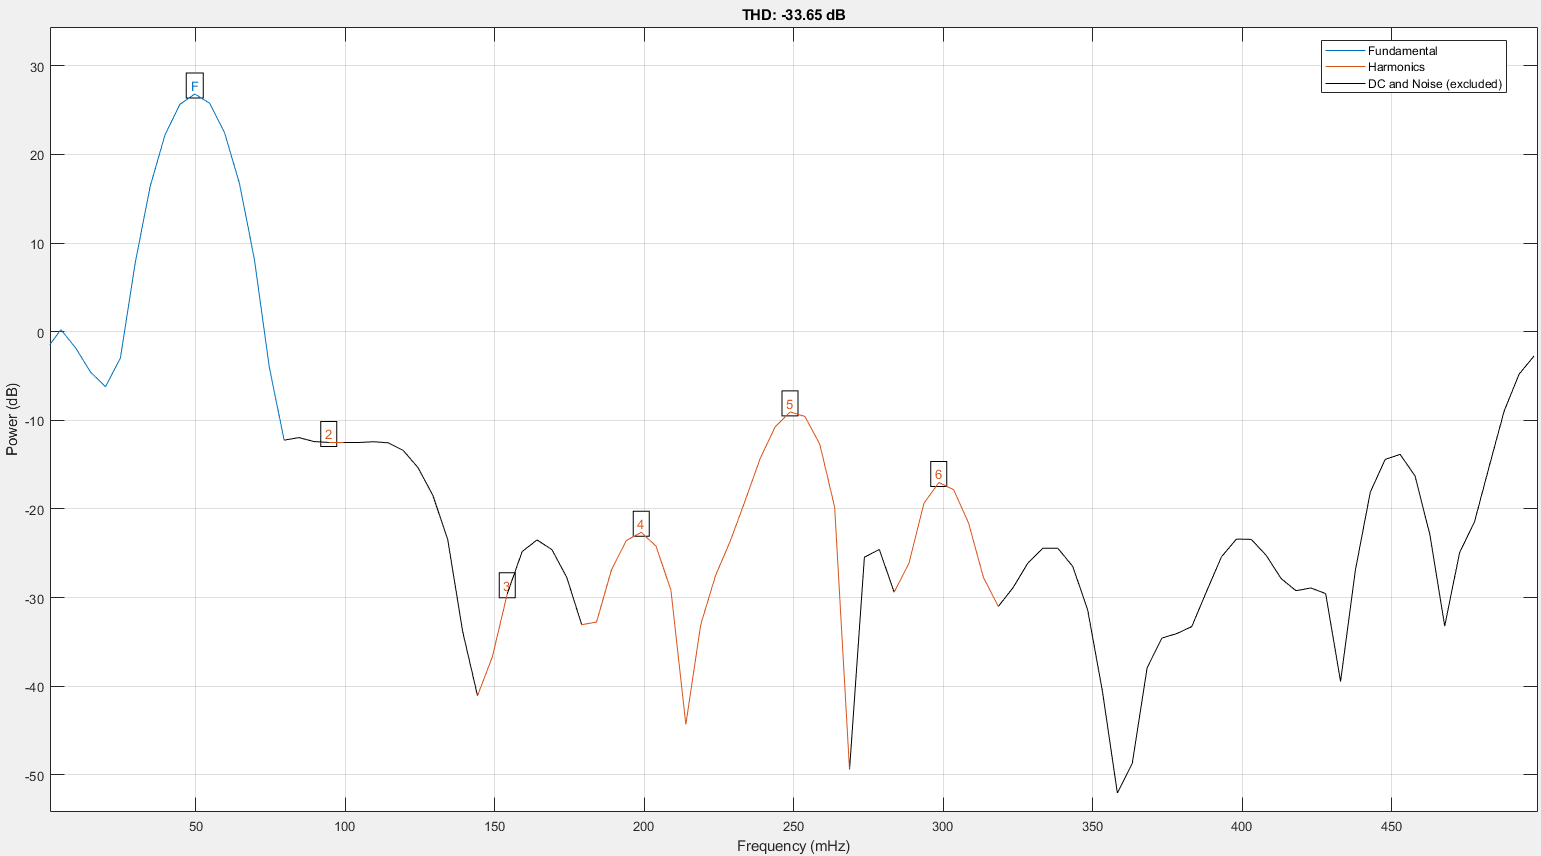
\includegraphics[width=15.5cm]{IMG3.png}
	\centering
\end{figure}

%% vedi i ths a 9, 8 e 7 bits